

% An example of a floating figure using the graphicx package.
% Note that \label must occur AFTER (or within) \caption.
% For figures, \caption should occur after the \includegraphics.
% Note that IEEEtran v1.7 and later has special internal code that
% is designed to preserve the operation of \label within \caption
% even when the captionsoff option is in effect. However, because
% of issues like this, it may be the safest practice to put all your
% \label just after \caption rather than within \caption{}.
%
% Reminder: the "draftcls" or "draftclsnofoot", not "draft", class
% option should be used if it is desired that the figures are to be
% displayed while in draft mode.
%
%\begin{figure}[!t]
%\centering
%\includegraphics[width=2.5in]{myfigure}
% where an .eps filename suffix will be assumed under latex, 
% and a .pdf suffix will be assumed for pdflatex; or what has been declared
% via \DeclareGraphicsExtensions.
%\caption{Simulation Results}
%\label{fig_sim}
%\end{figure}

% Note that IEEE typically puts floats only at the top, even when this
% results in a large percentage of a column being occupied by floats.


% An example of a double column floating figure using two subfigures.
% (The subfig.sty package must be loaded for this to work.)
% The subfigure \label commands are set within each subfloat command, the
% \label for the overall figure must come after \caption.
% \hfil must be used as a separator to get equal spacing.
% The subfigure.sty package works much the same way, except \subfigure is
% used instead of \subfloat.
%
%\begin{figure*}[!t]
%\centerline{\subfloat[Case I]\includegraphics[width=2.5in]{subfigcase1}%
%\label{fig_first_case}}
%\hfil
%\subfloat[Case II]{\includegraphics[width=2.5in]{subfigcase2}%
%\label{fig_second_case}}}
%\caption{Simulation results}
%\label{fig_sim}
%\end{figure*}
%
% Note that often IEEE papers with subfigures do not employ subfigure
% captions (using the optional argument to \subfloat), but instead will
% reference/describe all of them (a), (b), etc., within the main caption.


% An example of a floating table. Note that, for IEEE style tables, the 
% \caption command should come BEFORE the table. Table text will default to
% \footnotesize as IEEE normally uses this smaller font for tables.
% The \label must come after \caption as always.
%
%\begin{table}[!t]
%% increase table row spacing, adjust to taste
%\renewcommand{\arraystretch}{1.3}
% if using array.sty, it might be a good idea to tweak the value of
% \extrarowheight as needed to properly center the text within the cells
%\caption{An Example of a Table}
%\label{table_example}
%\centering
%% Some packages, such as MDW tools, offer better commands for making tables
%% than the plain LaTeX2e tabular which is used here.
%\begin{tabular}{|c||c|}
%\hline
%One & Two\\
%\hline
%Three & Four\\
%\hline
%\end{tabular}
%\end{table}


% Note that IEEE does not put floats in the very first column - or typically
% anywhere on the first page for that matter. Also, in-text middle ("here")
% positioning is not used. Most IEEE journals use top floats exclusively.
% Note that, LaTeX2e, unlike IEEE journals, places footnotes above bottom
% floats. This can be corrected via the \fnbelowfloat command of the
% stfloats package.

\section{Research}
\label{sec:research}
\IEEEPARstart{B}{efore} the application prototype is built, composing components of \emph{Android} applications are introduced in this chapter. In addition, it is shown why the MVP approach may improve app development and what MVP actually is.
% MVP applied to Android Apps

\subsection{Concepts \& Components of Android Applications}

Building \emph{Android} applications requires several core components of the \emph{Android} SDK to be used. This section gives a short overview and explanation of important components used in the implementation of the prototype created for this paper.

\textbf{Activity}: An application typically consists of one or more activities. An activity fills the whole screen of the device and can be compared to a \emph{window} in a classic desktop application. The official \emph{Android} SDK documentation \cite{SDKActivities} defines an activity as \enquote{an application component that provides a screen with which users can interact in order to do something}.
There is a defined lifcycle, which all activity objects share and follow -- the creation, start, resume, pause, stop and the destruction of an activity object. This lifecycle is managed by \emph{Android} itself, meaning application developers must not manually create or destroy activity objects.

\textbf{Fragment}: Fragments split more complex parts of an activity's user interface into several smaller sub-components. Fragments are also used to encapsulate reusable parts of the user interface, which for example need to appear in multiple activities. The official documentation of the \emph{Android} SDK defines a fragment as follows \cite{SDKFragments}:

\begin{quote}
A Fragment represents a behavior or a portion of user interface in an Activity. You can combine multiple fragments in a single activity to build a multi-pane UI and reuse a fragment in multiple activities.
\end{quote}

\textbf{Intent}: Intents are objects used for communication with the \emph{Android} system. An example would be the start of an activity: an intent must be created including some information to identify, which activity should be started. The intent will be handed over to the \emph{Android} system, which will create and start a corresponding activity. In the official SDK documentation, an intent is defined as \enquote{a messaging object you can use to request an action from another app component} \cite{SDKIntents}.

\subsection{Common Android Development Approach}
As a result of strong interrelations between its building components, the \emph{Android} system manages most of its components by itself. Given the complexity and interaction between these as well as the general structure, the framework steers developers toward handling tasks in common ways. In order to help developers understand the structure of the framework, code examples and component explanations are provided in \cite{SDKComponents}.

Since the building components are managed by the system and dependent on the implementations, one aspect that is inherently difficult is \emph{testability}. It is a challenge to divide business logic from the framework as it needs to react to certain system events -- like activity destruction, which may be forced by the system at any point in time and need to be appropriately handled by the developer.

Other common difficulties developers face lie with the \emph{maintainability} and \emph{extensibility} of their software. Given the \emph{Android} framework, its many components and classes that enable communication between these compontents, the structure often gets cluttered -- especially in larger application projects. For example, \emph{ListView}s\footnote{Component to \enquote{display a list of scrollable items}. \cite{SDKListView}} need \emph{Adapter}\footnote{Class to \enquote{bridge between AdapterView and the underlying data}. \cite{SDKAdapter}} to display their content, which in turn might use \emph{Loader}s\footnote{Component that \enquote{performs asynchronous loading of data}. \cite{SDKLoader}} and \emph{Cursor}s\footnote{Interface class providing access to results of database queries. \cite{SDKCursor}} to fetch the data to display.

In addition \emph{portability} is a problem as business logic that is strongly intertwined when developing for the \emph{Android} platform cannot easily be ported to other platforms.


\subsection{MVP: Passive View or Supervising Controller?}

Today, when we talk about MVP, we are talking about two different types: \emph{Supervising Controller} \cite{FowlerSupervisingController} and \emph{Passive View} \cite{FowlerPassiveView}. Fowler retired the classic MVP approach in 2006 \cite{FowlerMvpRetirementNote} and introduced those two implementations -- see Figure \ref{fig:mvp}.

\begin{figure}[!t]
\centering
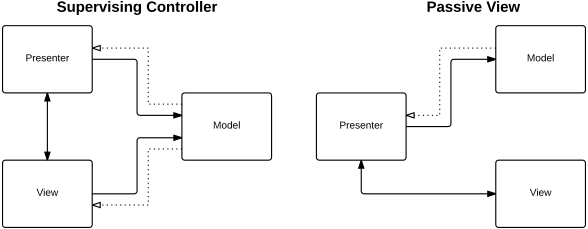
\includegraphics[width=0.5\textwidth]{mvp}
\caption{Supervising Controller and Passive View}
\label{fig:mvp}
\end{figure}

The \textbf{Supervising Controller} approach splits the User Interface in two components: a \emph{Presenter} and \emph{View} – like the classical MVP approach. The \emph{Model} can communicate changes to the \emph{View} using an Observer pattern (indirectly shown as dotted lines in Figure \ref{fig:mvp}). The \emph{View} can make direct changes to the model. In most cases this is done by simple mappings and \emph{Data Binding} capabilities provided by UI frameworks. Any user input is handled by the \emph{Presenter}. It determines how those interactions affect the underlying \emph{Model}. In addition, it handles complex view logic operations i.e. to prepare the model data for the view layer or vice versa, to transform the user input to fit the model requirements.

In contrast to the Supervising Controller, the \textbf{Passive View} totally separates the \emph{View} from the \emph{Model}. There is no direct or indirect interaction between them -- see Figure \ref{fig:mvp}. Interactions between \emph{View} and \emph{Model} is done exclusively via the \emph{Presenter}. This approach reduces the \emph{View} to an absolute minimum by using the \emph{Presenter} to handle all user input events, to update the \emph{Model} based on user interactions as well as to channel \emph{Model} changes back to the \emph{View}. As a result, the \emph{View} is made completely passive and is no longer responsible for updating itself from the \emph{Model}.

The primary driver for \emph{Passive View} is testing. This concept allows testing to be focused on the \emph{Presenter} without needing any interaction with the chosen UI framework.
